%%This is the evaluation part, int includes the following parts.
% <1> Evaluation Metrics, explain the measurements chosen for this experiments
% <2> Test Platform in KNIME, introduced before so we don't really need to repeat it here
% Firstly, we validate our methods and make sure it works for the properties.. Then using the whole data to test the weights tend and also, if it handled the real life data. 
% <3.1> validation part to check the methods work for those situations, but not necessary;; Then big data test to show property to handle those situations. 
% <3> Test Cases Design, the parameters we want to compare, the cases
%   ==> synthetic data
%   ==> Real life data
%   ++ Data to test the property
In this chapter, we evaluate the proposed repair techniques based on the quality of repaired models. At first, we define the evaluation criteria. Next, we briefly introduce the test platforms KNIME and relevant ProM plugins tools. Then, we conduct two kinds of tests. One is based one the demo example proposed in the Section \ref{sec:demo} part, and the other is based on real life data. 
\section{Evaluation Criteria}
% First talk about our data and our model, then choose the confusion matrix as one measurements. But we should review the traditional measuremtns on process mining before introducing the confusion matrix. but we should also focus on the accuracy part and f-score.
We evaluate the repair techniques based on the quality of repaired models with respect to the given event logs. In process mining, there are four quality dimensions generally used to compare the process models with event logs. 
\begin{itemize}
	\item Fitness. It quantifies the extent how well the model reproduces traces in the event log which is used to build the model.   
	\item Precision. It quantifies the extent how the discovered model limits the comletely unrelated behaviors that maybe show up in the event log. 
	\item Generalization. It addresses the over-fitting problem when a model strictly matches to only seen behaviors but is unable to generalize the behaviors which are not seen in the event log. 
	\item Simplicity. It captures the model complexity. According to Occam's razor principle, the model should be as simple as possible.
\end{itemize}
% How to come to confusion matrix?? 
The four traditional quality criteria are proposed in the environment where only positive instances are available. Therefore, when it comes to the model performance, where negative instances are also possible, the measurement metrics need to be adjusted. 

With labeled traces in the event log, the repaired model can be seen as a binary prediction model where the positive instances are supported while the negative ones are rejected. Consequently, the model evaluation becomes a classifier evaluation and confusion matrix is applied in our experiments.

% Describe its features and some derived measurements. 
Confusion matrix has a long history to evaluate the performance of a  classification model. A confusion matrix is a table with columns to describe the prediction model and rows for actual classification of data.  As seen as a binary classifier, the repaired model produces four outcomes according to the confusion matrix -- true positive, true negative, false positive and false negative, which is shown in the Table \ref{tab:cm}.
\begin{itemize}
	\item True Positive (TP): The execution allowed by the process model has a positive performance outcome.
	\item False Positive (FP): The execution allowed by the process model has a negative performance outcome.
	\item True Negative (TN): The negative instance is blocked by the process model.
	\item False Negative (FN):The positive instance is blocked by the process model.
\end{itemize} 
% confusion matrix
\begin{table}[]
	\caption{Confusion Matrix}
	\label{tab:cm}
	\begin{tabular}{ll|c|c|}
		\cline{3-4}
		&                   & \multicolumn{2}{c|}{repaired model}                                               \\ \cline{2-4} 
		\multicolumn{1}{l|}{}                                                                         &                   & \multicolumn{1}{l|}{allowed behaviors} & \multicolumn{1}{l|}{not allowed behaviors} \\ \hline
		\multicolumn{1}{|l|}{\multirow{2}{*}{\begin{tabular}[c]{@{}l@{}}actual \\ data\end{tabular}}} & positive instance & TP                                    & FN                                        \\ \cline{2-4} 
		\multicolumn{1}{|l|}{}                                                                        & negative instance & FP                                    & TN                                        \\ \hline
	\end{tabular}
\end{table}
Various measurements can be derived from confusion matrix. According to our application, the following criteria are chosen. Generally, there is a trade-off between the quality criteria. So the measurements below are only used to evaluate specific aspects of repair techniques.
\begin{itemize}
	\item Recall. It represents the true positive rate and is calculated as the number of correct positive predictions divided by the total number of positive instances.
	\[Recall = \frac{TP}{TP + FN}\]
	\item Precision. It describes the ability of the repaired model to produce positive instances.
	\[Precision = \frac{TP}{TP + FP }\]
	%\item specificity. In opposite with recall, it measures the true negative rate.
	%\[Specificity = \frac{TN}{TN + FP}\]
	\item Accuracy. It is the proportion of true positive and false results to the total results. In our case, it measures how well a model correctly allows the positive instances or blocks the negative instances.
	\[Accuracy = \frac{TP+TN}{TP+TN+FP+FN}\]
	\item F-score is is the harmonic mean of precision and recall.
	\[F_1 = \frac{2*Recall*Precision}{Precision + Recall}\]
\end{itemize}

\section{Experiment Platforms}
KNIME, as a scientific workflow analytic platform, supports automating the workflow testing, which helps us repeat experiments efficiently. Yet, the integration of traditional process mining plugins into KNIME is out of our capability due to the time limit. Therefore, partial experiments with current repair techniques are still conducted in ProM. 
\subsection{KNIME}
% this section describes how KNIME supports automatic test, FlowVariable and optimization parts of it.
KNIME supports automating workflow for testing mainly through the following mechanisms. 
\begin{itemize}
	\item Loop control structure. KNIME provides a bunch of control nodes which support re-executing workflow.  Two nodes \emph{Loop Start} and \emph{Loop End} explicitly express the beginning and end of a loop structure, where the workflow between those two nodes is the loop body and is executed recursively in a fixed number, or until certain conditions are met. In our test, we repeat our repair techniques for different parameter settings by applying loop structure into KNIME workflow.
	\item Flow variables. Flow variables are used inside a KNIME workflow to parameterize node settings dynamically. By introducing flow variables into loop body, tests with different settings are able to conduct automatically.
\end{itemize}
Furthermore, there are nodes provided by KNIME to optimize the value of some parameters with respect to a cost function. As long as the cost function is provided, KNIME is able to automatically optimize the corresponding parameters. 

\subsection{ Experiments with ProM Plugins}
Due to the frequent exceptions on the plugin for repair techniques in \cite{dees2017enhancing}, we exclude tests with this repair method  and conduct experiments with the following types. 
\begin{itemize}
	\item \textbf{Type 1} \textbf{Inductive Miner} bases only on the positive event log to discover a model. The default setting with infrequent variant and noise threshold 20\% is chosen. Later, the mined model is checked on the labeled event logs with positive and negative instances. This method is abbreviated as IM.
	\item \textbf{Type 2} \textbf{Repair Model} from \cite{fahland2015model} is applied on the positive event log to discover a model. The default setting of this plugin is chosen. Later, the mined model is checked on the labeled event with positive and negative instances. This method is abbreviated as Fahland, named after the name of the main author.
	\item \textbf{Type 3} \textbf{Dfg-Repair from our thesis} is applied on the labeled event log with positive and negative instances. Default setting  for the control parameters is 1.0 while the parameters to generate Petri nets from the directly-follows graph are set as the same as experiment Type 1.  Later, the repaired model is evaluated on the labeled data. 
\end{itemize}

\section{Experiment Results}
Our experiment contains two main parts. One is to verify if our method overcomes the limits of current repair algorithms. This experiment is based on the synthetic data and models in Section \ref{sec:demo}. The other experiment is based on real life data, in order to test the feasibility of our repair techniques.
%For convenience,we refer the repair methods in \cite{fahland2015model} by the main auther's name Fahland, and the repair techniques in \cite{dees2017enhancing} as Dees. The Inductive Miner is abbreviated as IM. Our method which built on directly-follows graph is denoted as Dfg-repair. 
 
\subsection{Test on Demo Example}
In this part, experiments are performed on the motivating examples which are listed in Section \ref{sec:demo}. Thereby, we are able to answer whether our repair method overcomes shortcomings of current techniques which are mentioned in the Section \ref{sec:demo}. 
\subsubsection{Answer to Situation 1}
\emph{Situation 1} shows the drawbacks of current repair methods \cite{fahland2015model} that unexpected behaviors are introduced into the model by adding subprocesses in the form of loops. Moreover, rediscover strategy with IM does not take the original model into account and generates a new model that deviates from the original model. 


Given the process model $M_0$ and the event log $L_1$, additional activities \textbf{x1} and \textbf{x2} in $L_1$ 
good performance and need to be added into the model $M_0$. Applying proposed repair techniques Dfg-repair, we obtain the  repaired model listed in Figure \ref{fig:demo_dfg_s1}. The parameters for our method are set in the following : weight for the existing model is 0.45, weight for positive examples is 1.0, the Inductive Miner for Infrequent is chosen and has a noise threshold of 20\%, which is the same setting as the rediscovery method by Inductive Miner in Section \ref{sec:demo}. 

As seen in Figure \ref{fig:demo_dfg_s1}, the subprocesses for \textbf{x1} and \textbf{x2} are added in a sequence with others. In this way, $M_{1.3}$ is able to reflect the deviations in positive instances while staying similar to the reference model $M_0$. Compared to techniques in \cite{fahland2015model}, it increases the precision without loops.
% we should give our confusion matrix result
\begin{figure}[htp]
	\centering
	\begin{subfigure}[b]{0.31\textwidth}
		\centering
		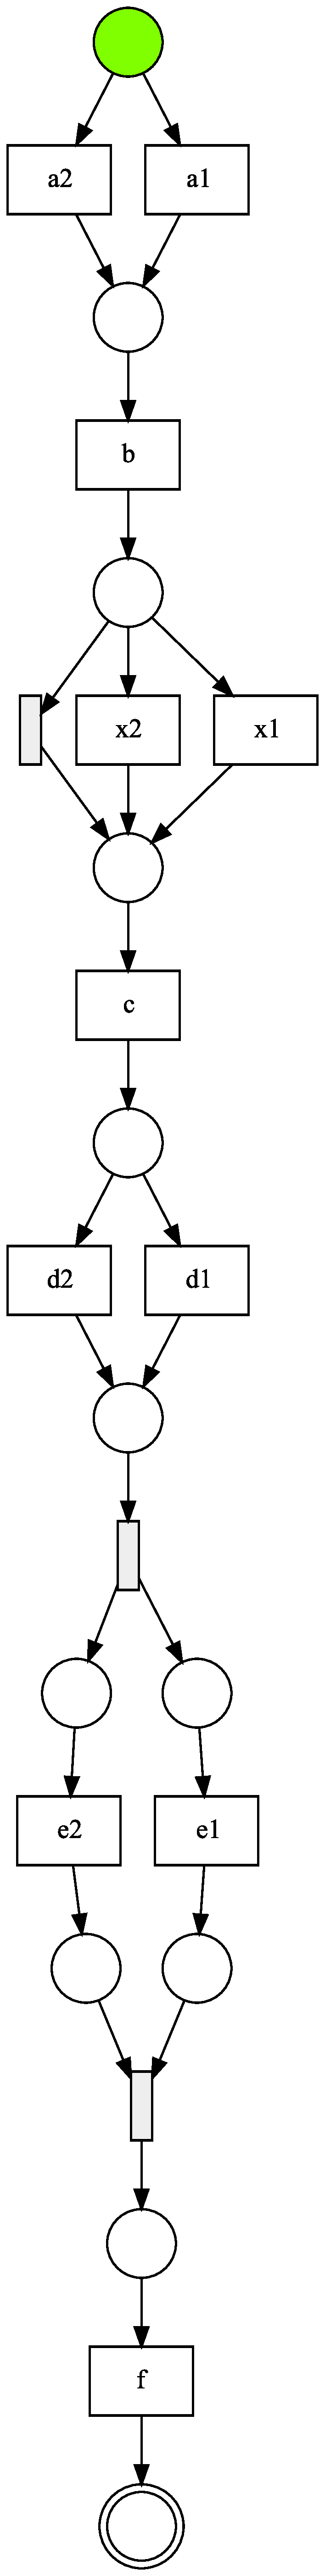
\includegraphics[width=0.75\linewidth, height=0.8\textheight]{figures/evaluation/PN-result-demo-s1-dfg.pdf}
		\caption{$M_{1.3}$ for situation 1}
		\label{fig:demo_dfg_s1}
	\end{subfigure}%
\quad
	\begin{subfigure}[b]{0.31\textwidth}
		\centering
		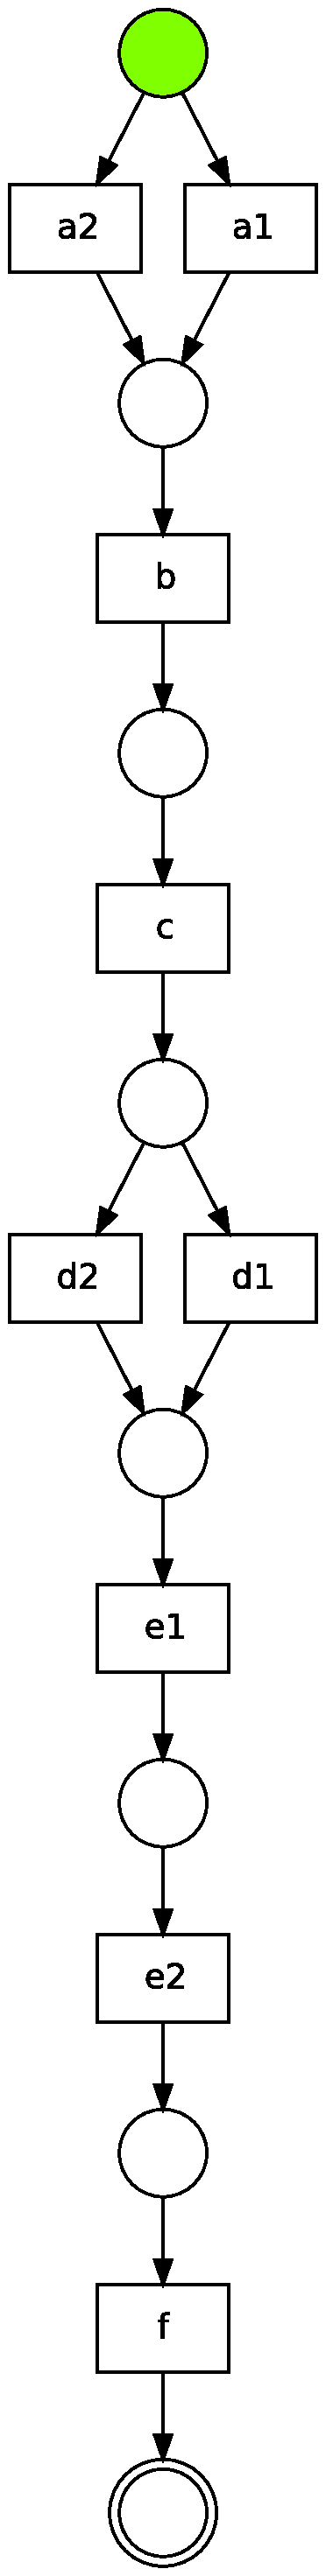
\includegraphics[ width=0.75\linewidth, height=0.8\textheight]{figures/evaluation/PN-result-demo-s2-dfg.pdf}
		\caption{$M_{2.3}$ for situation 2}
		\label{fig:demo_dfg_s2}
	\end{subfigure}
 \quad
\begin{subfigure}[b]{0.32\textwidth}
	\centering
	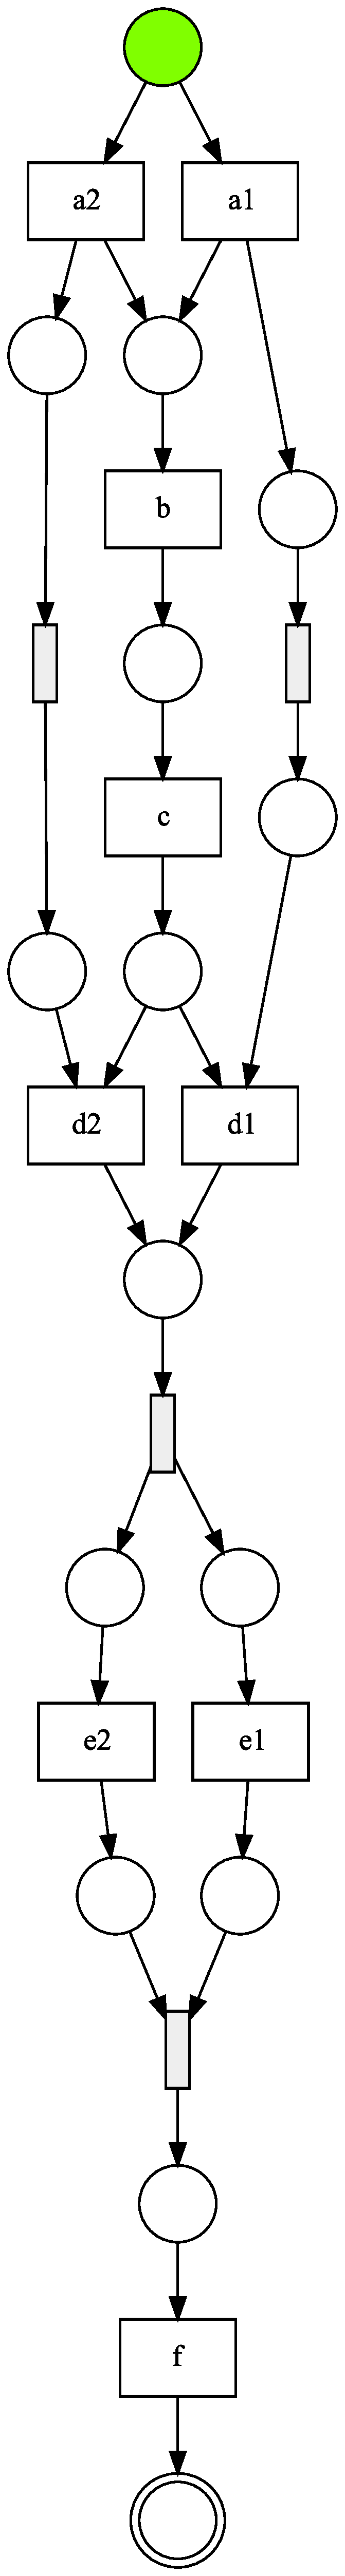
\includegraphics[ width=0.75\linewidth, height=0.8\textheight]{figures/evaluation/PN-result-demo-s3-dfg.pdf}
	\caption{ $M_{3.3}$ for situation 3}
	\label{fig:demo_dfg_s3}
\end{subfigure}
	\caption[Repaired models with Dfg-repair based on motivating examples]{repaired models with our techniques for situations 1, 2 and 3 in Section \ref{sec:demo} part. The green place is the initial marking of the Petri net and the doubled place is the final marking.}
	\label{fig:demo_dfg}
\end{figure}
\subsubsection{Answer to Situation 2}
Situation 2 describes the inability of current repair methods, i.e., fitting traces with negative performance outcomes cannot be used to repair a model. 
% some explaination about the situation.
The execution order of \textbf{e1, e2} affects the performance outcomes and \textbf{e1} is expected to be placed before \textbf{e2}. Without negative information, the repaired models have the same structure as the reference ones, because the execution of \textbf{e2} before \textbf{e1} also brings  the positive outcomes. 

If we apply our repair methods on the model $M_0$ and event log $L_2$, with 1.0 for all control weights, and the same Inductive Miner-Infrequent with noise 20, the repaired model $M_{2.3}$ is obtained. In $M_{2.3}$, \textbf{e1} is executed before \textbf{e2}. It shows that our method is able to incorporate the negative information and balance the forces from the existing model, positive and negative instances. 

\subsubsection{Answer to Situation 3}
% Conclusion part
Situation 3 concerns long-term dependencies in Petri nets, which is not handled in current repair and rediscovery techniques. As observed in the event log, there exists long-term dependencies set, $LT=\{ a1\rightsquigarrow d1, a2\rightsquigarrow d2\}$.  By adding long-term dependencies as expected in Figure \ref{fig:demo_s3_expected}, precision and accuracy increase, as the model limits activity selection and blocks the negative behaviors due to free execution of xor branches. Yet none of the current repair and rediscovery techniques are able to detect and add long-term dependencies in the Petri net. 

In our repair techniques, long-term dependencies is taken into account. With the Petri net $M_0$ and event log $L_3$, our methods produces the repaired model $M_{3.3}$ with long-term dependencies. Two silent transitions that are used to explicitly represent long-term dependencies can be deleted with post process to reduce the redundant silent transitions and places. After reduction, our repaired model is simplified as the model $M_{3}$. 
\subsubsection{Comparison with Confusion Matrix}
In this section, we list the evaluation results of the repaired models based on confusion matrix. In Table \ref{tab:demo-result}, for Situation 1 with only positive instances, the repair techniques give the same confusion matrix result. However,  $M_{1.2}$  with loops implicates a lower precision. In Situation 2, with current techniques or rediscovery methods in IM, the model stays the same as the reference  model $M_0$. Since no negative instance is rejected, the recall is 1 but precision is below 0.6.  In comparison, Dfg-repair uses the negative instances and adjusts the model correspondingly. Therefore, the repaired model $M_{2.3}$ has  higher precision, accuracy and F1 score. In Situation 3 with long-term dependencies, our method succeeds to detect and add the  long-term dependencies in the model. In this way, no false positive or false negative instances are in the confusion matrix, and the repaired model holds the highest values for all listed measurements.
\begin{table}[h]
	\centering
	\caption{Test Result on BPI15-M1 data}
	\label{tab:demo-result}
	\resizebox{\textwidth}{!}{
		\begin{tabular}{lll|llllllll|}
			\hline
			\multirow{2}{*}{\thead{Situation}} & \multirow{2}{*}{\thead{method} }                &    \multirow{2}{*}{\thead{Generated \\ model}}       & \multicolumn{8}{l|}{ \thead{confusion matrix metrics}}                                \\
			\cline{4-11}
			&  &     &
			\thead{TP}  & \thead{FP} & \thead{TN}  & \thead{FN}  & \thead{recall} & \thead{precision} & \thead{accuracy} & \thead{F1}             \\
			\hline
			S1      & IM              & $M_{1.1}$ & 50 & 50 & 0 & 0 & 1   & 0.5     & 0.5     & 0.667               \\
			S1     & Fahland              & $M_{1.2}$   & 50   & 50  &0     &0     & 1   & 0.5     & 0.5     & 0.667               \\
			
			S1      & Dfg-repair              &    $M_{1.3}$    &  50   &  50  &  0  &    0 &  1   & 0.5     & 0.5     & 0.667               \\
			
			\hline
			S2      & IM/Fahland              & $M_0$   & 60    & 45   &  0  & 0    &  1     &    0.571       & 0.571         &  0.727   \\
			
			S2      & Dfg-repair              & $M_{2.3}$      & 50    &   5 &   40  & 10    &  0.833      &   0.909        &  0.857         &  0.870      \\
			
			\hline
			S3     & IM/Fahland             & $M_{0}$   & 100    & 100   &  0   &  0   &  1.0      &   0.5        &   0.5       &  0.667    \\
			
			S3      & Dfg-repair             & $M_{3.3}$       &  100   &   0 &  100   &  0   &  1      &   1        &  1        &   1     \\
			\hline         
	\end{tabular}}
\end{table}

In conclusion, our proposed method is able to conquer shortcomings of current techniques mentioned in the Section \ref{sec:demo}. It avoids the loops for additional activities as the work in \cite{fahland2015model}. By incorporating the negative information, it is able to output the repaired model which blocks the negative behavior. Additionally, it detects and adds long-term dependencies into model. In this way, the repaired model has better recall, and accuracy.

\subsection{Test on Real Life Data}
% here we will list all the data here but before describe the test data
We choose publicly available event logs from the BPI challenge 2015 and build a data set from them to test the feasibility of proposed repair techniques.
\subsubsection{Data Description}
The data set for BPI Challenge 2015 contain 5 event logs which are provided by five Dutch municipalities respectively. Those event logs describe the building permit application around four years. We choose them as the basis to build our test data due to the following reasons.
\begin{itemize}
	\item The event logs hold attributes as potential KPIs to classify traces. Attribute \textbf{SUMleges} which records the cost of the application is a candidate to label traces as positive or negative if its value  is over the threshold. Furthermore, we take the throughput time of the application as another potential KPI. 
	In a word, this data set provides us information to reasonably label traces.
	\item The five event logs describe an identical process, but include deviations caused by the different procedures, regulations in those municipalities. Also, the underlying processes have changes over four years.
	This data set gives us a basic process but also allows deviations of the actual event logs and predefined process. This builds the experiments environment for repair techniques.
\end{itemize}
We conduct our experiments on those event logs. However, due to the time limits, we only managed to get the results on experiments with the event log \textbf{BPIC15\_1.xes.xml}. This event log includes 1199 cases and 52217 events in 398 classes. We preprocess the event log and get a proper subset of data as our user case.  
\begin{table}[h]	
	\caption{Test event log from real life data BPI15-1}
	\label{tab:event-log}
	\begin{tabular}{|l|l|l|l|l|}
		\hline
		Data ID & Data Description                                & Traces Num & Events Num & Event Classes \\ \hline
		D1      & \makecell{heuristic filter  \\ with 40 }                     & 495        & 9565       & 20             \\ \hline
		D2      & \makecell{apply heuristic filter \\ on D1 with 60      }     & 378        & 4566       & 12            \\ \hline
		D3.1    & \makecell{classify on SUMleges;  \\ values below 0.7 as positive} & 349        & 6744       & 20             \\ \hline
		D3.2    & \makecell{classify on SUMleges;  \\ values above 0.7 as negative }& 146        & 2811       & 20             \\  \hline
		D3.3    & union of D3.1 and D3.2                             & 495        & 9596       & 20             \\ \hline
		D4.1    & \makecell{ classify on throughput time;  \\ values below 0.7 as positive} & 349        & 6744       & 20             \\ \hline
		D4.2    & \makecell{classify on throughput time;  \\ values above 0.7 as negative} & 146        & 2811       & 20            \\ \hline
		D4.3    & union of D4.1 and D4.2                             & 495        & 9596       & 20           \\ \hline
	\end{tabular}
\end{table}

We filter the raw event log by \textbf{\emph{Filter Log By Simple Heuristic}} in ProM with the following setting: 40\% threshold for the start, end  activities and the other events. We get the event log $D1$. After this, we calculate the throughput time for each trace and add it as a trace attribute \textbf{throughput time}. 
Then we classify traces according to  \textbf{SUMleges} and  \textbf{throughput time} separately. When our performance goal is to reduce the cost of application, if \textbf{SUMleges} of one trace is over 70\% of the whole traces, this trace is treated as negative, else as positive. The similar strategy is applied on the attribute \textbf{throughput time}. A trace with \textbf{throughput time} higher than 70\% of all traces is considered as a negative instance. Following this preprocess, we gain event logs in Table \ref{tab:event-log} available for our tests. 


\begin{table}[htp]
	\caption{Generated reference models for test}
	\label{tab:ref-models}
	\resizebox{\textwidth}{!}{
	\begin{tabular}{|llll|lllllllll|}
		\hline
		\multirow{2}{*}{\thead{Model\\ ID}} & \multirow{2}{*}{\thead{Used \\Data}} & \multirow{2}{*}{\thead{Setting}}  &  
		\multirow{2}{*}{\thead{Event\\Class}} & \multicolumn{9}{c|}{\thead{Confusion Matrix Evaluation}}                     \\ 
		\cline{5-13}
		&                                                                           &                                                                             &                                                                            &Data & TP & FP & TN & FN & recall & precision & accuracy & F1 \\ \hline
		M1                                                                      & D1                                                                        & \makecell[l]{IM-infrequent: \\ Noise Setting: 20} & 20                                                                         & D3.3 & 112   & 40   & 106   & 237   & 0.321       &0.737           &   0.440       &   0.447 \\
		
		&                                                                      & &                                                                          & D4.3 & 131   &  21  &  128  & 215   & 0.379       & 0.862           & 0.523          & 0.526    \\
		
		\hline
		M2                                                                      & D1                                                                        & \makecell[l]{IM-infrequent: \\ Noise Setting: 50} & 20                                                                         & D3.3 & 106   & 39   &  107  & 243    & 0.304        &  0.731         &0.430          &0.429    \\
		
		&                                                                      & &                                                                          & D4.3 & 125   &   20 & 129   &221    &    0.361    & 0.862           & 0.513          &0.509    \\
		\hline
		
		M3                                                                      & D2                                                                        & \makecell[l]{IM-infrequent: \\ Noise Setting: 20} & 12                                                                         &D3.3 &  0  & 0   & 146   & 349   & 0       &NaN           &    0.295      & 0   \\
		
		&                                                                      & &                                                                          & D4.3 &  0  & 0   & 149   & 346   & 0       & NaN           &  0.301        &0    \\
		\hline 
		
		M4                                                                      & D2                                                                        & \makecell[l]{IM-infrequent: \\ Noise Setting: 50} & 12                                                                         &D3.3 &  0  &  0  &  146  & 349   & 0       & NaN           &     0.295     & 0\\   
		&                                                                      & &                                                                          & D4.3 &  0  & 0   & 149   & 346   & 0       & NaN           &  0.301        &0    \\
		
		\hline
	\end{tabular}
 }
\end{table}
Based on the filtered data, we derive corresponding Petri nets as reference process models. The Table \ref{tab:ref-models} lists the models with different settings. \textbf{IM-infrequent} is one variant of Inductive Miner working on event logs with infrequent traces. \textbf{Noise} is set as the threshold to filter out infrequent traces. After mining reference models, we compare them with  corresponding event logs to get the basis lines for later evaluation.
% should we explain the data and the model, they are different with old files!!
% Please add the following required packages to your document preamble:
% \usepackage{multirow}

As seen in Table \ref{tab:ref-models}, the reference models do not apply well to the corresponding event logs. M3 and M4 reject all positive instances while M1 and M2 have lower recall and F1 score.  The models are in demand to reflect the reality better, and also to enforce the positive instances and avoid negative instances. 
\subsubsection{Test Result}
% we don't need to transfer page to landscape view, because we have many rows too.
Three types of repair techniques which are \textbf{IM}, \textbf{Fahland} and \textbf{Dfg-repair}, are applied on preprocessed event log set in Table \ref{tab:event-log} and models from Table \ref{tab:ref-models}. The repaired model is evaluated on the alignment-based conformance checking with cost function 1 for all deviations. The experiment results are listed in the Table \ref{tab:rl-result}. For better understanding, we give the details of one experiment set which is conducted with the reference model M3 and event log D3.1 and D3.3.  

Figure \ref{fig:rl_ref} displays the reference model M3, which has 0 TP and 0 FP compared to D3.3. It implies that M3 leads to no positive performance outcomes. Firstly, the rediscovery techniques -- Inductive Miner for infrequent traces with noise threshold 20\% is used on the positive event log D3.1 to rediscover a model. The generated model is shown in Figure \ref{fig:rl_IM}, which has changed a lot compared to the original model M3 as shown in the Figure \ref{fig:rl_ref}. After getting the generated model, we compare it with labeled event log D3.3 and compute the confusion matrix criteria as a baseline for our comparison. 

After applying the Fahland's repair techniques from \cite{fahland2015model}, the reference model M3 is repaired as Figure \ref{fig:rl_fahland}. With duplicated transitions, loops and silent transitions, the repaired model is more complicated than the reference model M3. When evaluating the repaired model with confusion matrix, we get 349 TP, 145 FP, 1 TN, and 0 FN, which leads to high recall. However, the principle of Fahland repair techniques is to add subprocesses for deviations in the model. Without consideration of eliminating negative behaviors, the repaired model is likely to damage the model precision and accuracy.

Dfg-repair techniques are firstly applied with the default setting, 1 for all control parameters. It results in a model with 0 TP, 0 FP, 146 TN, and 349 FN,  which contrasts the result by Fahland repair techniques. This might be caused by that the forces from the existing model and negative instances exceed the positive force, and block behaviors with positive outcomes. 

As a comparison, we change the control parameter setting to 0.5 for the existing model, 1 for the positive instances, 0.5 for the negative instances. After repeating the experiment, the confusion matrix changes to 131 TP, 63 FP, 83 TN, and 217 FN, while recall increases from 0 to 0.378, accuracy from 0.294 to 0.428, and F1 from 0 to 0.485. Apparently, the quality is improved due the the new setting. The possible reason is that three forces are balanced more properly for the repaired model.

% here to fix the evaluation from last step!! Better to give a good result on it!! Put it aheda before the whole result, and then organize it later.
\begin{figure}[htp]
	\centering
	\begin{subfigure}[b]{0.45\textwidth}
		\centering
		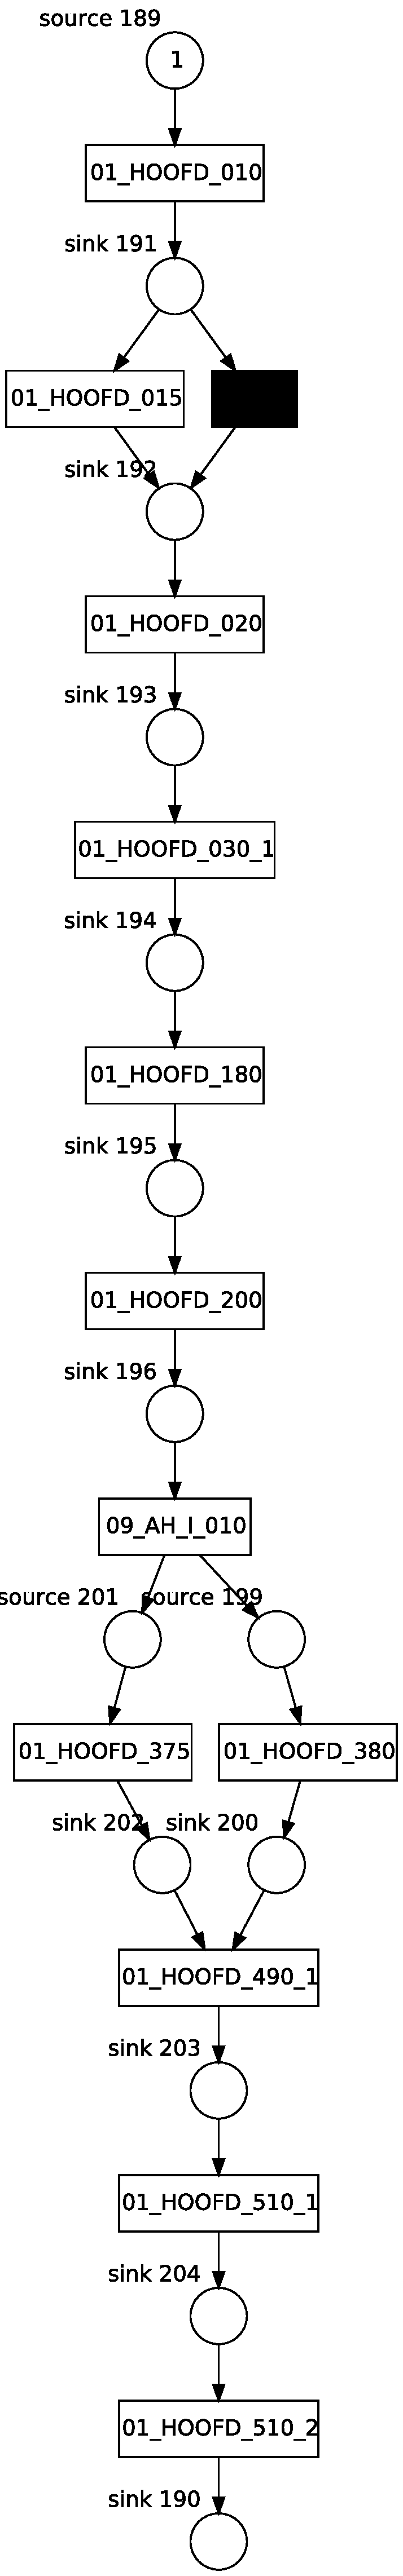
\includegraphics[width=0.7\textwidth, height=0.9\textheight]{figures/evaluation/BPI_1_40_M3_figure.pdf}
		\caption{reference model M3}
		\label{fig:rl_ref}
	\end{subfigure}%
\quad
\begin{subfigure}[b]{0.45\textwidth}
	\centering
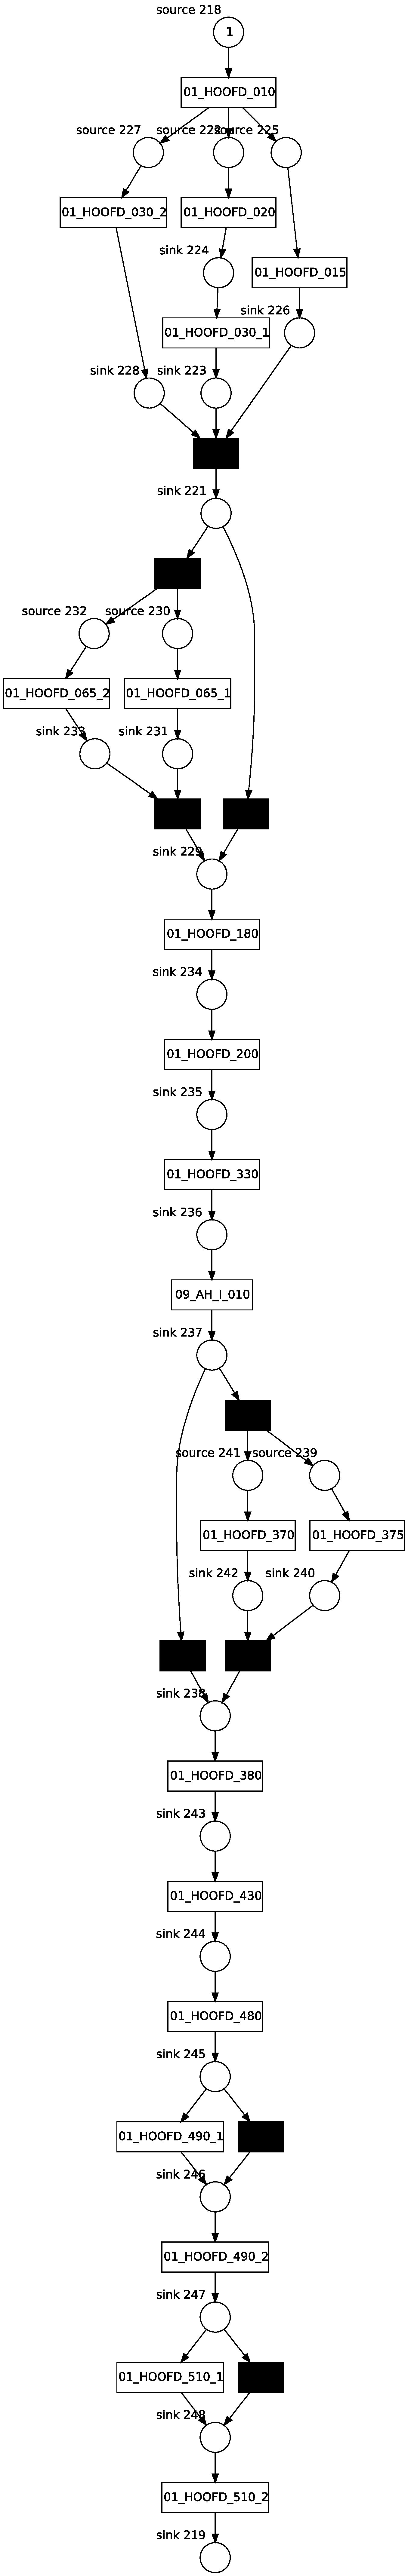
\includegraphics[width=1.0\textwidth, height=0.9\textheight]{figures/evaluation/PN-result-D4-1-IM20-pos.pdf}
\caption{repaired model with IM}
\label{fig:rl_IM}
\end{subfigure}%
\caption[Reference model M3 and the rediscovered model for it with IM]{The left model is the reference model M3. The rediscovery algorithm IM generates a new model based on the positive instances which is shown on the right side.}
\end{figure}

%two figures to show the reference models and IM generated model
\begin{figure}[htp]
	\centering
	\begin{subfigure}[b]{0.55\textwidth}
		\centering
		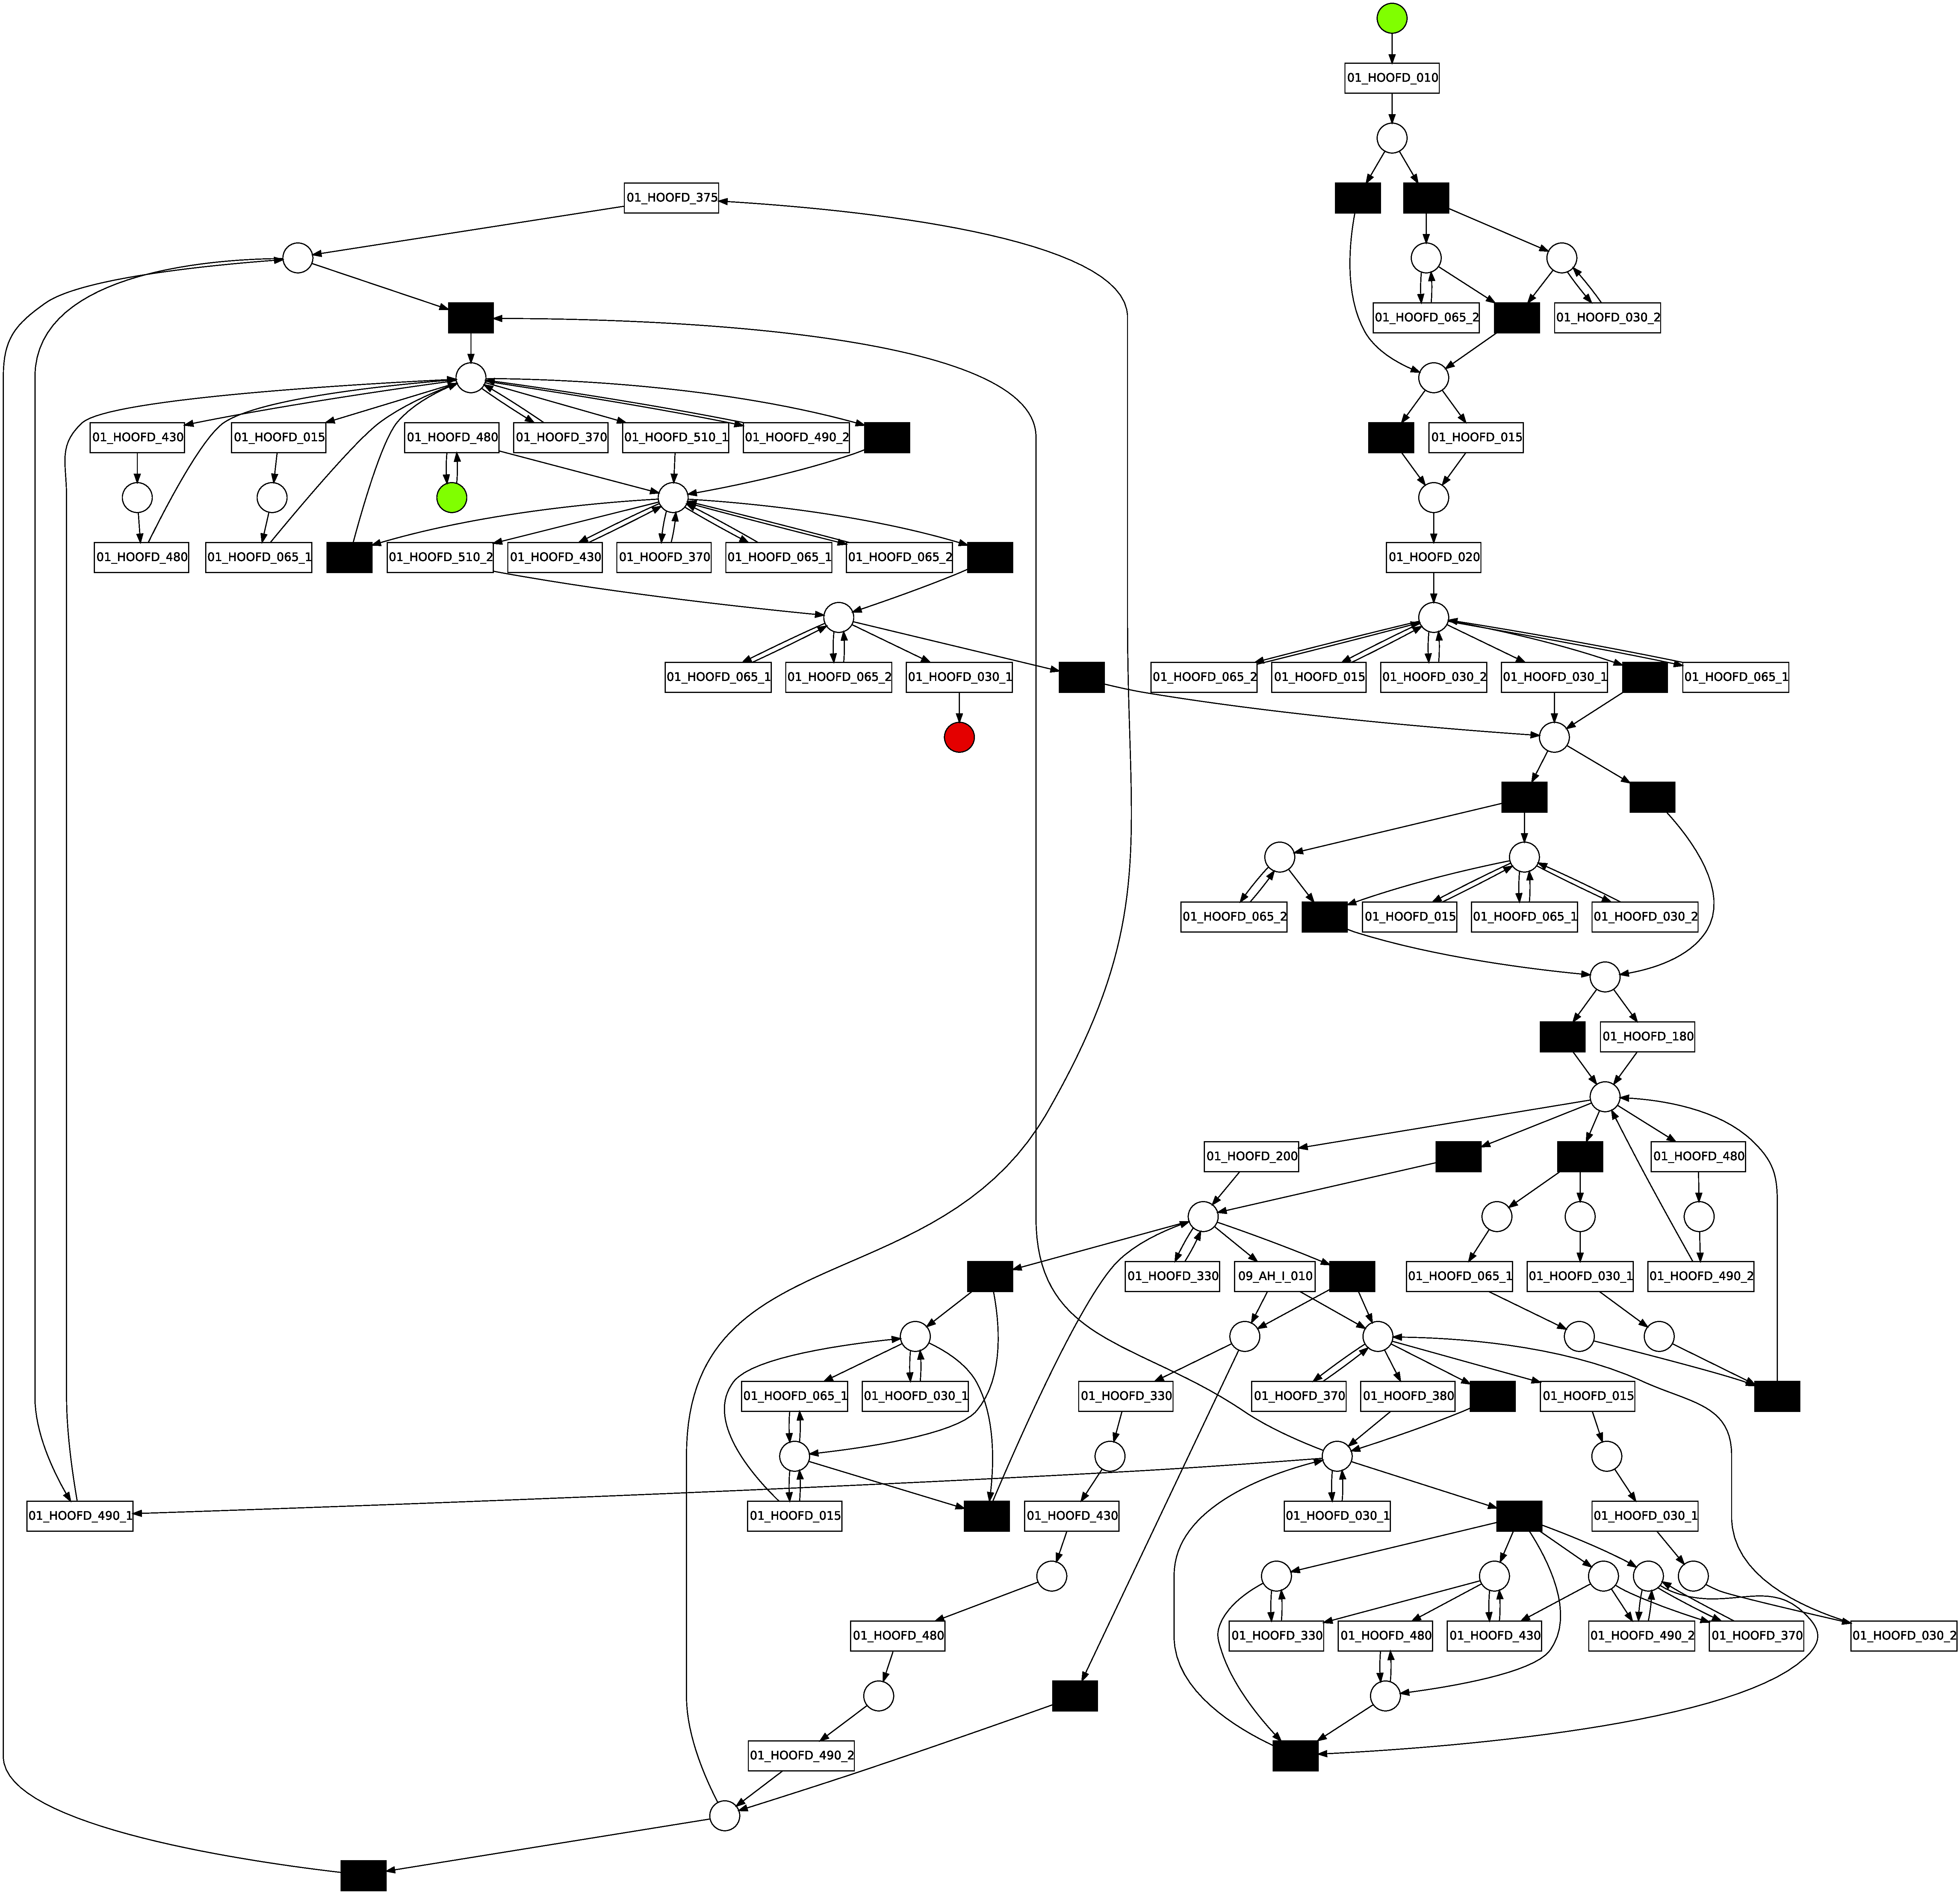
\includegraphics[width=1.0\textwidth, height=0.9\textheight]{figures/evaluation/PN-result-D4-3-M3-fahland-new.pdf}
		\caption{repaired model with Fahland}
		\label{fig:rl_fahland}
	\end{subfigure}%
	\begin{subfigure}[b]{0.43\textwidth}
		\centering
		
\includegraphics[width=.9\textwidth, height=0.9\textheight]{figures/evaluation/PN-result-D4-3-M3-dfg-05-1-05.pdf}
		\caption{repaired model with Dfg-repair}
		\label{fig:rl_dfg}
	\end{subfigure}
	\caption[Repaired models with Fahland and Dfg-repair techniques]{Repaired model for $M_3$ based on event log D3.1 with positive instances for Fahland's repair techniques  while event log D3.3 with both positive and negative instances for Dfg-repair. The weight setting for Dfg-repair is 0.5 for the existing model, 1 for positive and 0.5 for negative instances. Default setting is chosen for Fahland's method.}
\end{figure}


\begin{table}[ht]
	\centering
	\caption{Test Results on BPI15-M1 data}
	\label{tab:rl-result}
	\resizebox{\textwidth}{!}{
		\begin{tabular}{lll|llllllll|}
			\hline
			\multirow{2}{*}{\thead{event \\ log}} & \multirow{2}{*}{\thead{reference \\ model} }                &    \multirow{2}{*}{\thead{method}}       & \multicolumn{8}{l|}{ \thead{confusion matrix metrics}}                                \\
			\cline{4-11}
			&  &     &
			\thead{TP}  & \thead{FP} & \thead{TN}  & \thead{FN}  & \thead{recall} & \thead{precision} & \thead{accuracy} & \thead{F1}             \\
			\hline
			D3.1      & -              & IM & 137 & 48 & 118 & 289 & 0.32   & 0.74      & 0.43     & 0.45                \\
			D3.1      & M1              & Fahland   & 343   & 136  &10     &6     &0.983        & 0.716           &   0.713       & 0.829         \\
			
			D3.3      & M1              & Dfg-repair:1-1-1       &  124   &  52  &  94   &    225 &   0.355     &     0.705      & 0.44         & 0.472            \\
			D3.3      & M1              & Dfg-repair:0.5-1-0.5       &  155   &  66  &  80   &    194 &   0.444     &     0.701     & 0.474         & 0.544            \\
			\hline
			D3.1      & M2              & Fahland   & 317    & 133   &   13  & 32    &  0.908      &    0.704       & 0.667         &  0.793   \\
			
			D3.3      & M2              & Dfg-repair:1-1-1       & 124    &   52 &   94  & 225    &  0.355      &   0.705        &  0.44         &  0.472      \\
			
			D3.3      & M2              & Dfg-repair:0.5-1-0.5       & 155    &   66 &   80  & 194    &  0.444      &   0.701        &  0.475         &  0.544      \\
			\hline
			D3.1      & M3              & Fahland   & 35    & 7   &  139   &  314   &  0.100      &   0.833        &   0.352       &  0.179    \\
			
			D3.3      & M3              & Dfg-repair:1-1-1       &  0   &   0 &  146   &  349   &  0      &   NaN        &  0.295       &   0      \\
			D3.3      & M3              & Dfg-repair:0.5-1-0.5       &  132   &   63 &  83   &  217   &  0.378      &   0.677        &  0.434        &   0.485      \\
			\hline
			
			D3.1      & M4              & Fahland   &  0   & 0  &  146   &  349   & 0       &   NaN        &   0.294      &  0.0         \\
			
			D3.3      & M4              & Dfg-repair:1-1-1       &  0   &  0  &   146  &  349   &  0     &      NaN     & 0.294        & 0   \\
			D3.3      & M4              & Dfg-repair:0.5-1-0.5       &  125   &  59  &   87  &  224   &  0.358     &      0.679     & 0.428        & 0.469   \\
			\hline
			D4.1      & -              & IM &  131   &  21  & 128    &  215   &    0.379    & 0.862           &   0.523       &    0.526     \\
			D4.1      & M1              & Fahland   &  325   &  133  &  16   & 21    &   0.939     &  0.710         &  0.689       & 0.808                \\
			
			D4.3      & M1              & Dfg-repair:1-1-1       &  139   & 36   & 113    &   207  &   0.402     &   0.794        &   0.509       &   0.534                   \\
			D4.3      & M1              & Dfg-repair:0.5-1-0.5       &  172   & 48   & 101    &   174  &   0.497     &   0.782       &   0.552       &   0.608                   \\
			\hline
			D4.1      & M2              & Fahland   & 325    &  130  & 19    &  21   & 0.939       &    0.714       &  0.695        &  0.811                \\
			
			D4.3      & M2              & Dfg-repair:1-1-1     &  139   & 36   & 113    &   207  &   0.402     &   0.794        &   0.509       &   0.534              \\
			D4.3      & M2              & Dfg-repair:0.5-1-0.5     &  172   & 48   & 101    &   174  &   0.497     &   0.782        &   0.552       &   0.608              \\
			\hline
			D4.1      & M3              & Fahland   & 10    &  20  & 129    &  336   & 0.029       &    0.333       &  0.281        &  0.053                    \\
			D4.3      & M3              & Dfg-repair:1-1-1       &  0   &  0  & 346    &  149   &  0      &   NaN        &   0.303       &  0       \\ 
			D4.3      & M3              & Dfg-repair:0.5-1-0.5       &  182   &  49  & 164    &  100   &  0.526      &   0.788        &   0.70       &  0.631      \\ 
			
			\hline
			D4.1      & M4              & Fahland   & 5    &  14  & 135    &  341   & 0.014      &    0.263      &  0.283        &  0.027                 \\
			
			D4.3      & M4              & Dfg-repair:1-1-1       &   0  & 0   &  346   & 149    &   0     &    NaN       &     0.303     &  0      \\  
			D4.3      & M4              & Dfg-repair:0.5-1-0.5       &   172  & 48   &  101   & 174    &   0.497     &    0.782       &     0.552     &  0.608      \\      
			\hline              
	\end{tabular}}
\end{table}
% add some analysis on them..

With overview of results in Table \ref{tab:rl-result}, Inductive Miner rediscovers a new model from the given positive instances, while the reference models are simply ignored. As a result, the generated models probably change a lot compared to the original models. With respect to confusion matrix, the rediscovered models have similar measurement values for M1 and M2 but higher measurements than the reference models M3 and M4.


Fahland's repair techniques from \cite{fahland2015model} tend to have high recall but low values for true and false negative on the M1 and M2. The possible reasons are that  (1) M1 and M2 benefit already the positive outcomes;  (2) after repairing those models  by adding subprocesses, more behaviors  are introduced into the model, which also allows the negative instances.   In contrast, on M3 and M4 which block all the positive instances, it has low recall, but high values for TN and FN. The structures of original models dominates the performance outcomes. Since M3 and M4 blocks all positive instances, if the repaired models retains the main structure, it  blocks the positive instances as well. 


Dfg-repair techniques uses control parameters to balance the forces from the existing model, positive and negative instances. Therefore, with different setting, Dfg-repair techniques repair the model in different ways. To address this phenomenon, besides the default setting with value 1 for all parameters, another setting with 0.5 for the existing model, 1 for the positive instances, 0.5 for the negative instances is used to conduct experiments.  Compared to the default setting, the setting with values 0.5, 1 and 0.5 results in models with higher recall, accuracy, and F1 score. The reasons behind might be that the force from negative instances affects model a lot, with the weight 1.0. It possibly blocks the behaviors which contribute to positive performance.  With lower value on it, the forces from the existing model, positive and negative are balanced better and the quality of the repaired model is improved. As an example, the experiments on D3.3 and M3, or D.3. and M4, which show the quality changes due to different settings.

Except for the weight for negative instances, the weights for the existing model and positive instances also affect the quality of repaired model. To investigate the effect of those weights on the repaired model, we conducts our experiments with the following settings.


Each of three control parameters for the existing model, positive and negative instances changes value from 0.0 to 1.0 with step 0.1. With this setting, directly-follows relation is generated. Afterward, the default setting of Inductive Miner Infrequent with noise threshold 20 is used to mine Petri nets from the generated directly-follows graph. In total, 1000 experiments are conducted with proposed Dfg-repair method. 
After filtering out the data with missing value NaN, we average the confusion matrix results fixed with the analyzed weight,  and draw plots to show the tendency of evaluation results on the weight for the existing model, positive and negative event logs, respectively. 

\begin{figure}[htb]
	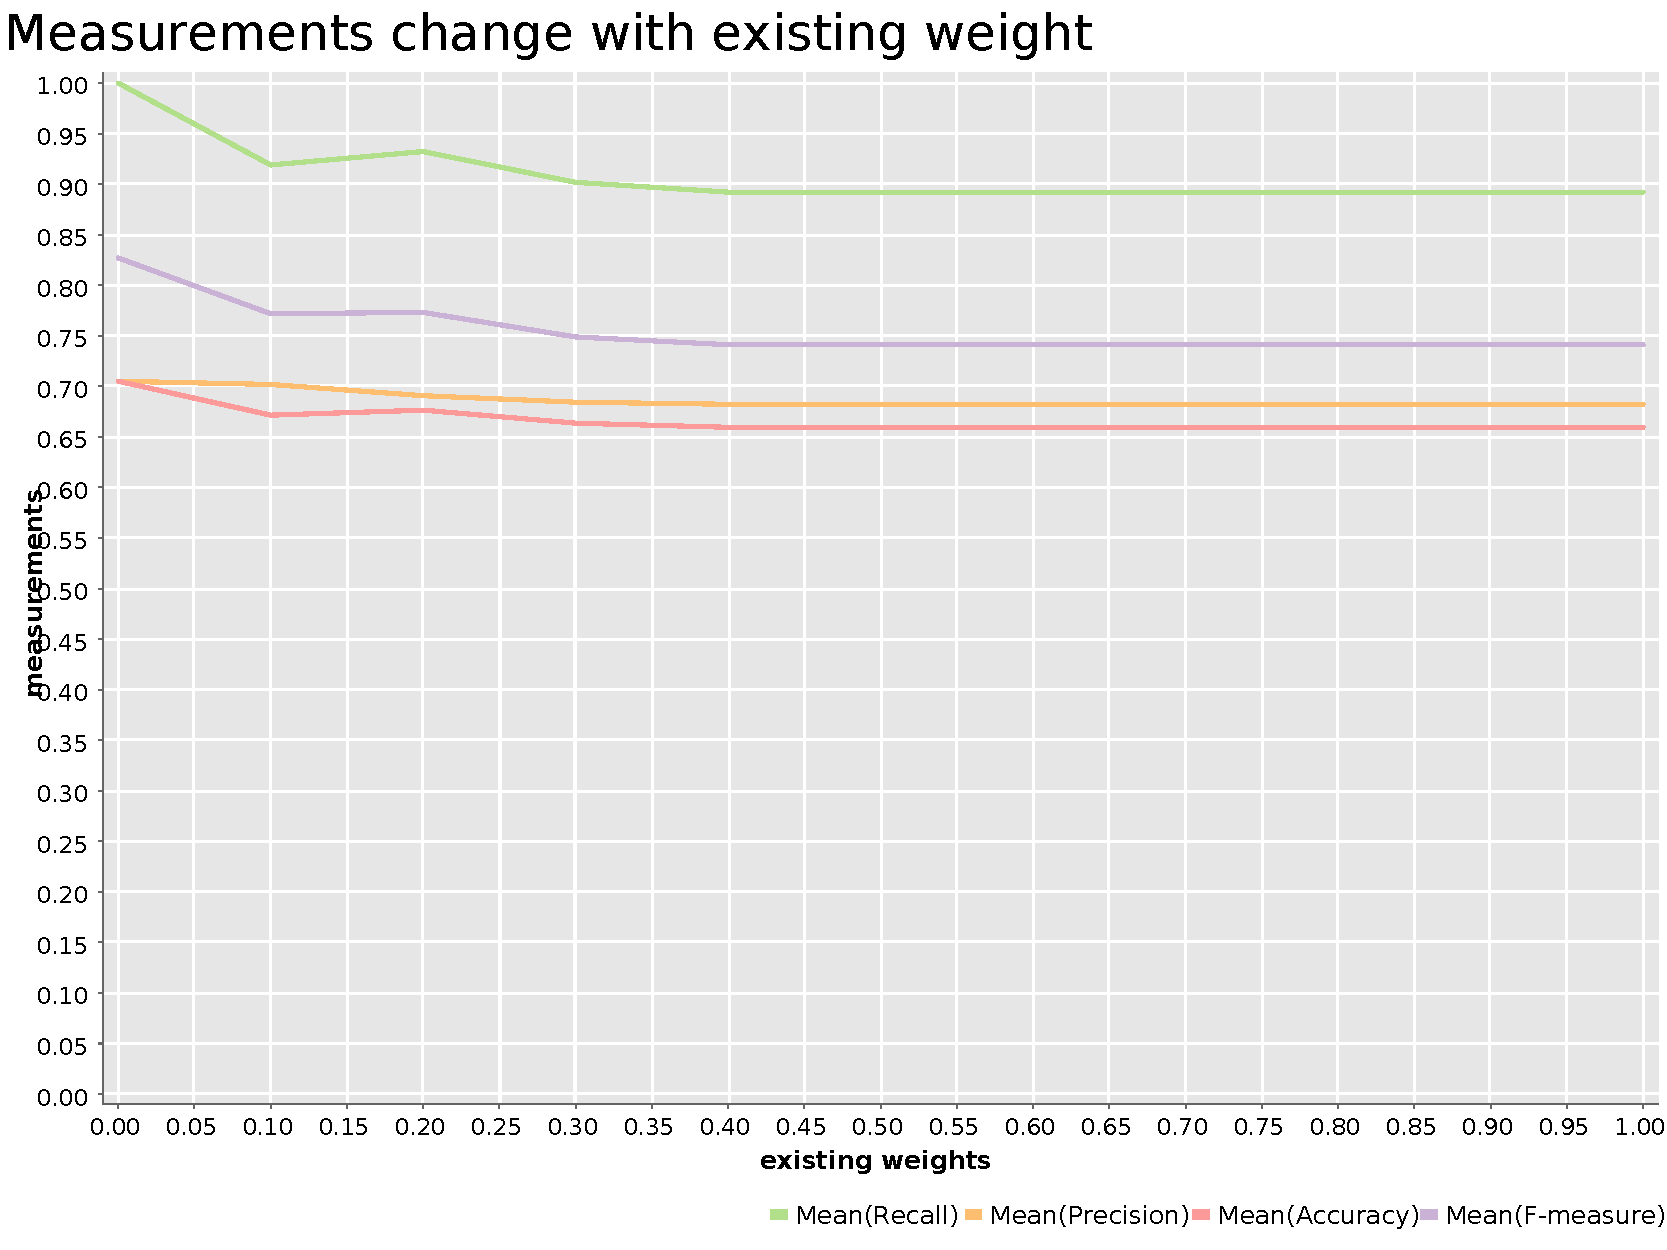
\includegraphics[width=\linewidth]{figures/evaluation/M3-D43-ext-weight-plot.pdf}
	\caption[Result tendency with weight for the existing model]{Result with weight for existing model on event log D3.3 and model M3.}
	\label{fig:ext-weight}
\end{figure} 
For the experiments on the Figure \ref{fig:ext-weight}, as the parameter for the existing model goes up, recall, accuracy and F1 go down firstly and then become stable. Because the reference model M3 tends to block positive behaviors  from model, with the weight for the existing model going up, the force to keep the model as M3 increases. Thereby, the repaired model fits less positive instances and the recall goes lower. 

\begin{figure}[htb]
	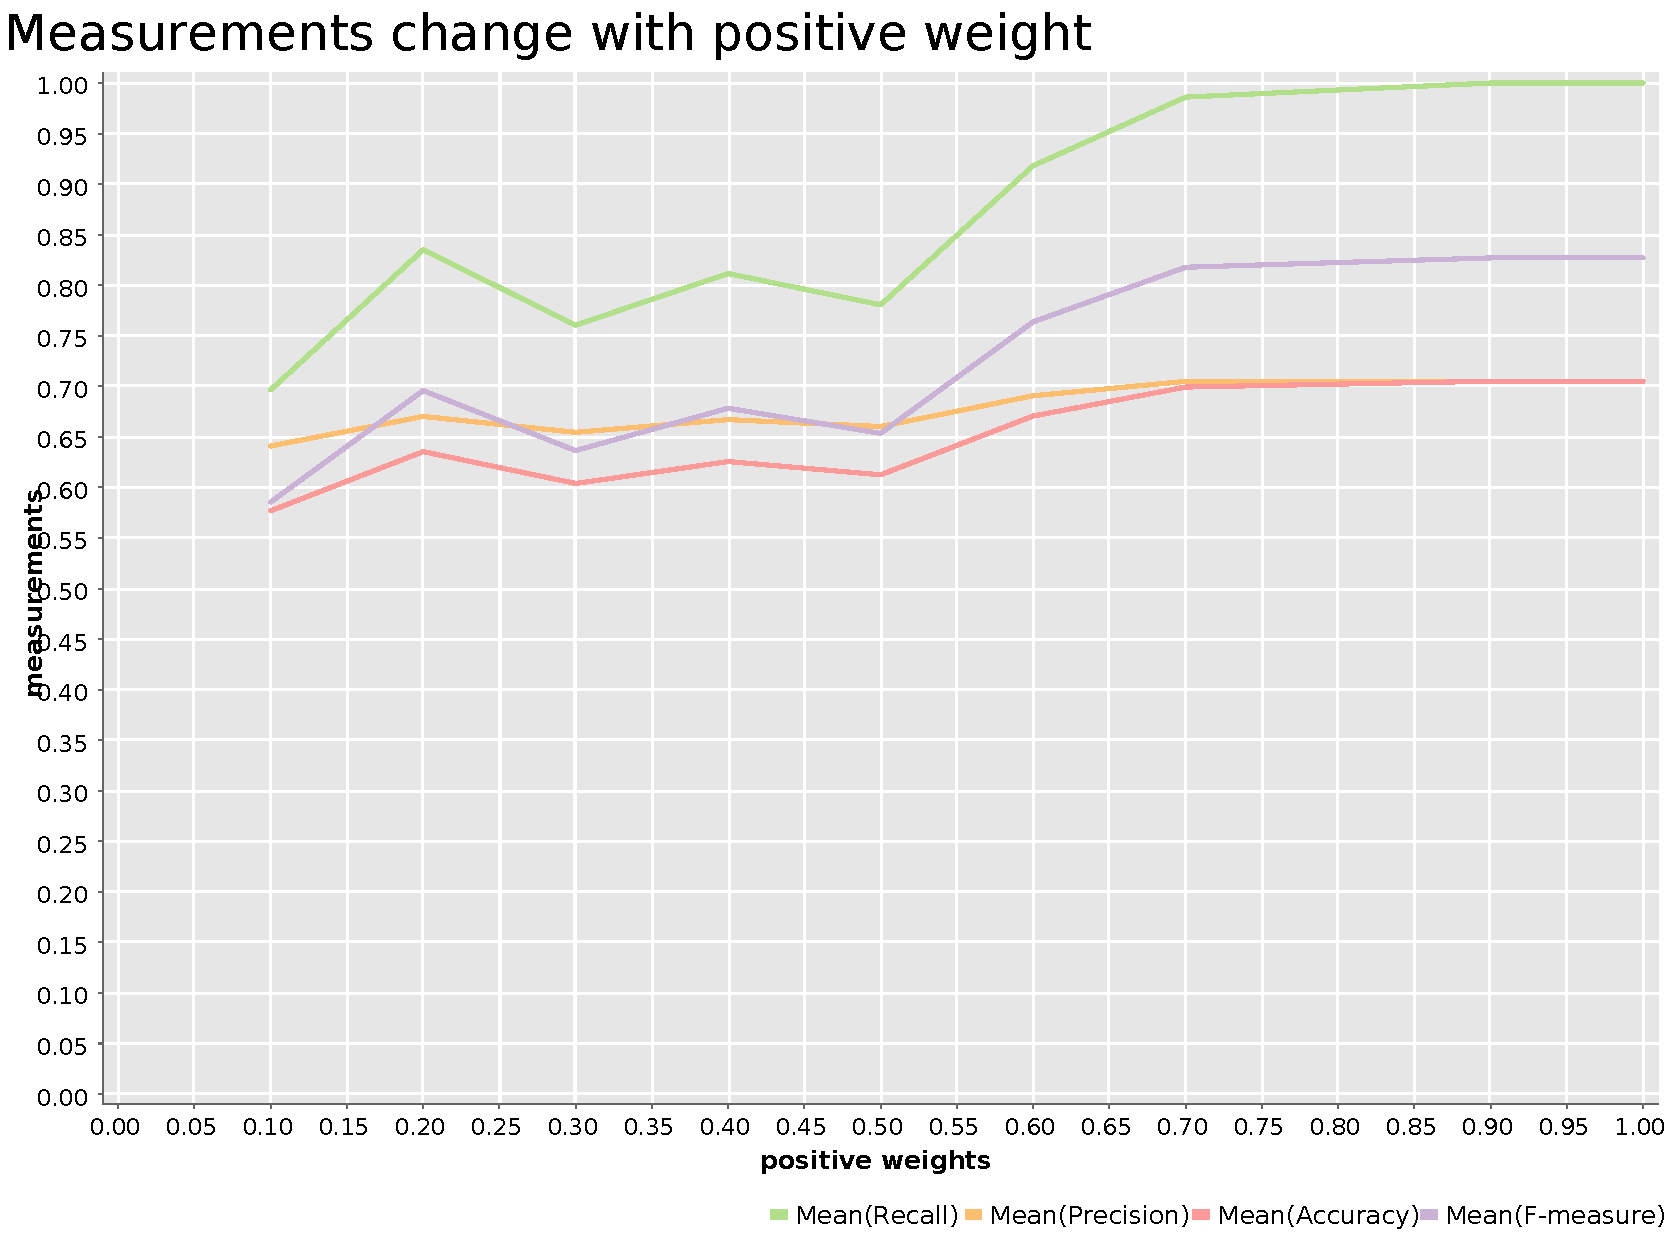
\includegraphics[width=\linewidth]{figures/evaluation/M3-D43-pos-weight-plot.pdf}
	\caption[Result tendency with weight for positive instances]{Result with weight for positive instance on event log D3.3 and model M3.}
	\label{fig:pos-weight}
\end{figure}
Figure \ref{fig:pos-weight} displays the tendency with the weight for positive event log. When the weight rises, recall, precision and accuracy increase. The reason might be the forces from the existing model and negative event logs tend to block the positive instances. With higher values, the force for the positive instances adjusts the model with better balance. Therefore, as the weight for positive event log increases, the repaired model allows more positive behaviors  and leads to the increase of all criteria related to confusion matrix.

\begin{figure}[htb]
	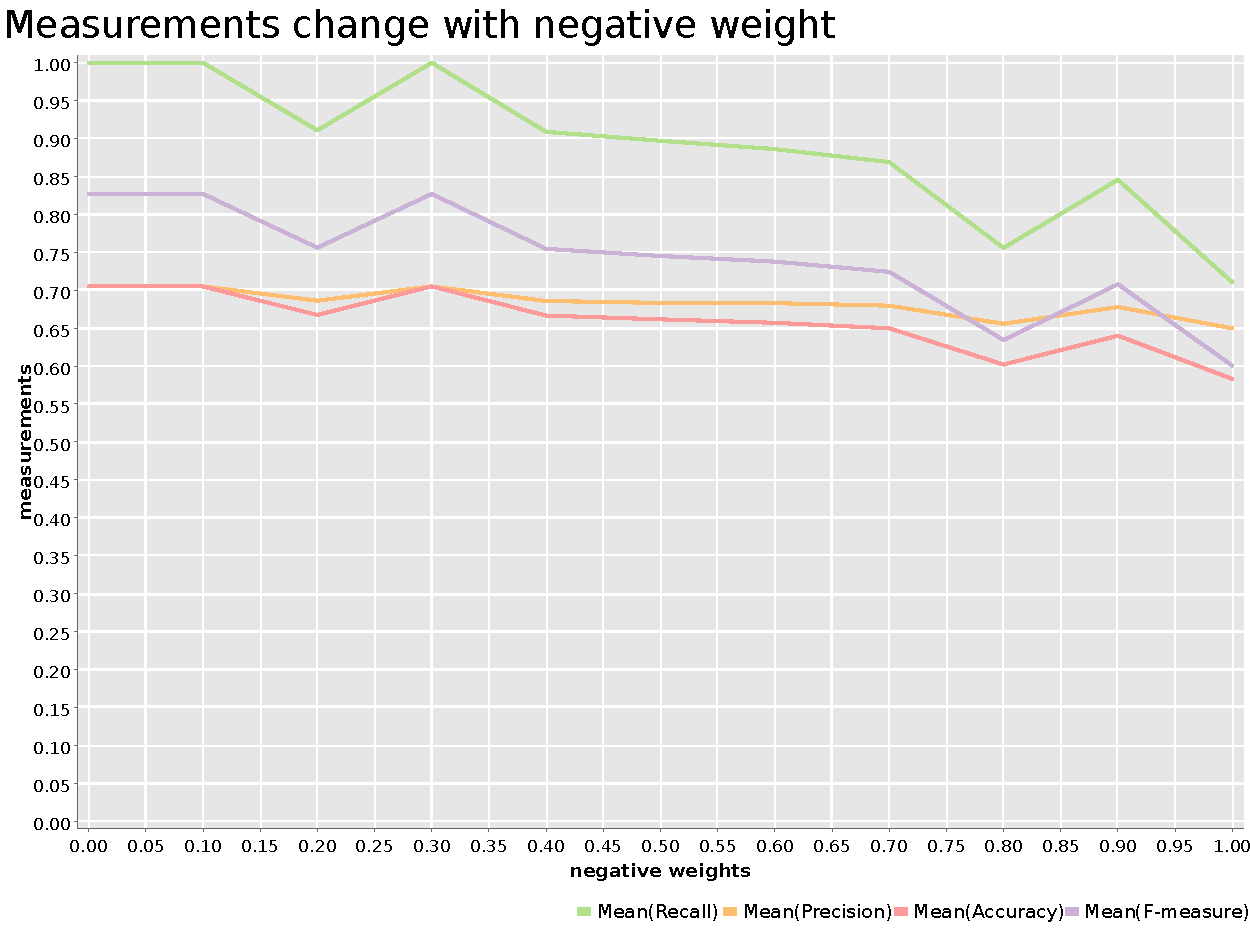
\includegraphics[width=\linewidth]{figures/evaluation/M3-D43-neg-weight-plot.pdf}
	\caption[Result tendency with weight for negative instances]{Result with weight for negative instance on event log D3.3 and model M3.}
	\label{fig:neg-weight}
\end{figure}
Figure \ref{fig:neg-weight} shows the tendency with the weight  for negative event log. With lower value, the weight leads to higher recall, precision and accuracy. The negative force is possibly over the force from positive event log. When the weight increases, behaviors which contribute to positive performance are likely to be deleted from the models. In this way, the measurements go down with the weight going up.

By applying our proposed method in the real life data, it is feasible to repair model in reality.   Compared to IM with the same rediscovery setting, Dfg-repair techniques are able to output models with higher recall, accuracy and F1 score. At the same time, it keeps the models as similar to the reference models, while IM simply ignores the reference models. Compared to Fahland repair techniques, which bring more behaviors into the model and cause high values with TP and FP, Dfg-repair techniques take negative information into account and are capable to produce models with higher values in TN. Moreover, the repaired models from Dfg-repair are simpler than the ones from Fahland repair techniques.  With observation, Dfg-repair also runs faster.  

Yet, we need to notice that the optimal control parameter setting differs in various situations. Trials are in demand to find the optimal setting for Dfg-repair techniques. 

